\chapter{要素技術}
本章では,本研究で用いた深層学習に関連した要素技術について述べる.

\section{Deep learning}
Deep learningは近年,自然言語処理など様々な分野で利用されている.
人間の脳におけるニューロンの構造を数理モデル(パーセプトロン)を用いて再現したニューラルネットワークを多層構造にすることで,
複雑なタスクの解決に必要な関数の表現力を高めたものである.
一般的な構造をFig. \ref{fig::network}示す.

\begin{figure}[h]
    \centering
    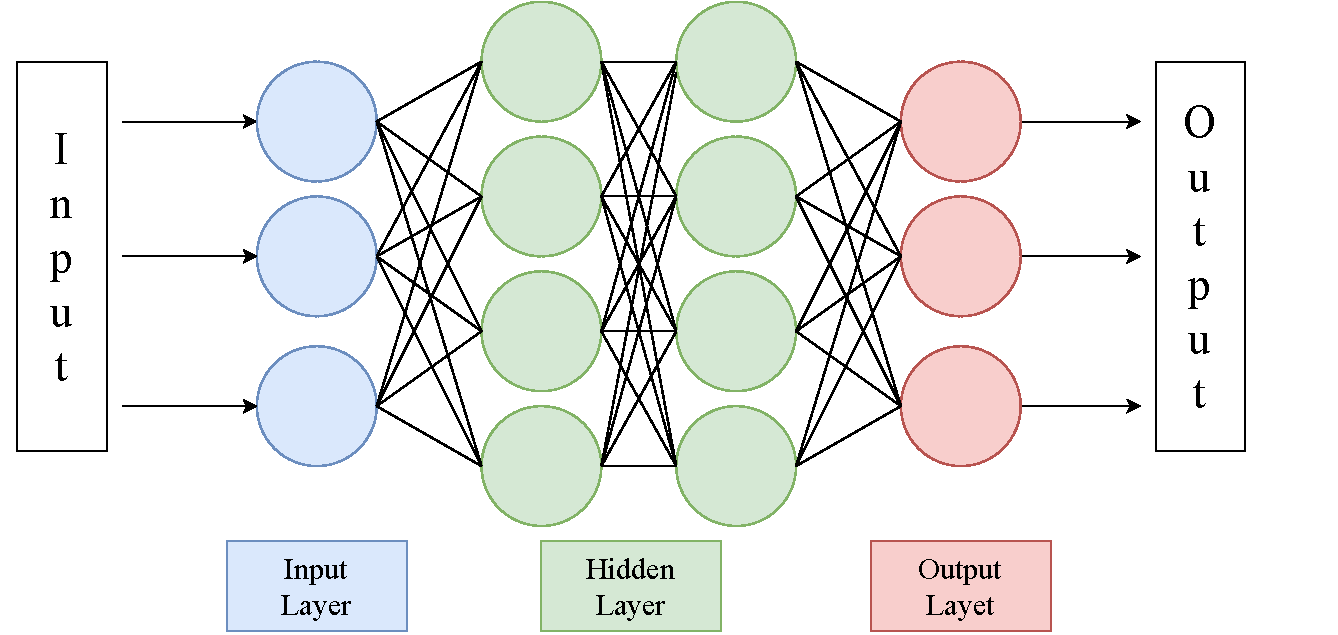
\includegraphics[width = 12cm]{./figs/net.pdf}
    \caption{Neual Network}
    \label{fig::network}
\end{figure}

\section{End-to-End学習}
End-to-Endとは「端から端まで」という,
Fig. \ref{fig::e2e}に示すように生データ(入力)から目的の結果(出力)を得るために必要な多段階の処理をNeusal Networkを用いて直接学習を行うものである.
例として,実世界における自動運転では人物や障害物などの物体認識,走行レーンの検出,経路計画,ステアリング制御
などの人間が設定した複数個のタスクを解く必要があるが,End-to-End学習では先程のタスクを人間が直接設定せずに
カメラ画像をニューラルネットワークに入力することで直接ステアリング操作を学習する.

\vspace{2.0zh}
\begin{figure}[h]
    \centering
    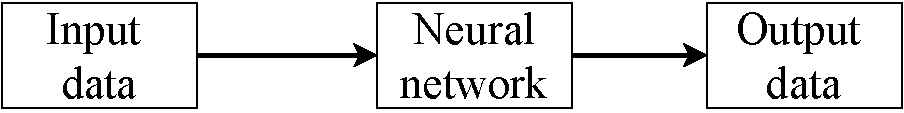
\includegraphics[width = 10cm]{./figs/e2e.pdf}
    \caption{Structure of End-to-End learning}
    \label{fig::e2e}
\end{figure}

\newpage
\section{Convolition Neual Network}
畳み込みニューラルネットワーク(convolutional neural network:CNN)は
画像認識や音声認識などの多次元の配列で表される複雑なデータを扱う処理へ用いられているニューラルネットワークである.
次のような特徴をもつ層で構成されている.

\begin{enumerate}
    \item 畳み込み層:入力データへフィルタ(カーネル)を用いて畳み込み演算を行うことで,特徴を抽出した特徴マップを取得する
    \item プーリング層:Maxプーリングなどの演算を用いて特徴マップのダウンサンプリングを行う
    \item 全結合層:畳み込み層,プーリング層で行った特徴を抽出したデータを一つのノードに
                      集約を行い,分類などの結果の出力を行う
\end{enumerate}


Krizhevskら\cite{Imagenet}はFig. \ref{fig::alex}で示すような3つの畳み込み層(convolutional layer),2つのプーリング層(pooling layer)
および 3 つの全結合層(fully connected layer)から構成したネットワークを用いて,
120万の高解像度画像を1,000の異なるクラスに分類をエラー率15.3\%で達成し,画像分類コンペティションであるILSVRC(ImageNet Large Scale Visual Recognition Competition)2012
で優勝をおさめた

\vspace{2.0zh}

\begin{figure}[h]
    \centering
    \includegraphics[width = 15cm]{./figs/alex.pdf}
    \caption{Alex net from \cite{Imagenet}}
    \label{fig::alex}
\end{figure}

